\documentclass[conference]{IEEEtran}

\usepackage[utf8]{inputenc}
\usepackage[spanish]{babel}
\usepackage{amsmath}
\usepackage{amssymb}
\usepackage{graphicx}
\usepackage{float}
\usepackage[siunitx, american]{circuitikz}
\usepackage{placeins}
\usepackage{array}

\graphicspath{{assets/}}

\IEEEoverridecommandlockouts
\raggedbottom

\begin{document}

\title{Momento Evaluativo 3\\
Métodos Sistemáticos de Análisis:\\
Supermallas y Análisis Nodal}

\author{

\IEEEauthorblockN{
1\textsuperscript{st} Kevin Ramírez Corrales
}

\IEEEauthorblockA{
\textit{Universidad Cooperativa de Colombia}\\
kevin.ramirezcorr@campusucc.edu.co
}

\and

\IEEEauthorblockN{
2\textsuperscript{nd} Mauro Jaramillo Zapata
}

\IEEEauthorblockA{
\textit{Universidad Cooperativa de Colombia}\\
mauro.jaramillo@campusucc.edu.co
}

\and

\IEEEauthorblockN{
3\textsuperscript{rd} Sofía Valero Loaiza
}

\IEEEauthorblockA{
\textit{Universidad Cooperativa de Colombia}\\
sofia.valero@campusucc.edu.co
}

}

\maketitle

\begin{abstract}
En este informe se desarrollan dos ejercicios de análisis de circuitos eléctricos utilizando los 
métodos de supermallas y análisis nodal. Se realizaron procedimientos matemáticos completos, 
simulaciones y comparación de resultados teóricos. Además, en el ejercicio de análisis nodal se 
implementó el circuito físicamente para verificar experimentalmente los valores obtenidos.
\end{abstract}

\begin{IEEEkeywords}
Circuitos eléctricos, análisis nodal, supermallas, leyes de Kirchhoff, 
corrientes de malla, voltajes nodales
\end{IEEEkeywords}

\section{Introducción}
El análisis de circuitos eléctricos es una herramienta fundamental en el estudio de sistemas 
electrónicos y eléctricos. Existen diferentes métodos que permiten determinar corrientes y voltajes 
dentro de un circuito de manera organizada y matemática.
En este trabajo se desarrollan dos técnicas importantes vistas durante el curso: el método de 
supermallas y el método de análisis nodal. Ambos procedimientos se apoyan en las Leyes de Kirchhoff 
y la Ley de Ohm para resolver circuitos resistivos de corriente continua.
Para cada ejercicio se realizaron cálculos matemáticos detallados y simulaciones computacionales con 
el fin de verificar la coherencia de los resultados obtenidos.

\section{Ejercicio 1: Método de supermallas}

\subsection{Planteamiento}

El circuito mostrado en la Fig.~\ref{fig:supermalla} debe resolverse utilizando el método de supermallas 
para encontrar las corrientes de malla $i_1$, $i_2$, $i_3$ e $i_4$, además de los voltajes $v_{x1}$ y 
$v_{x2}$.

\begin{figure}[H]
\centering
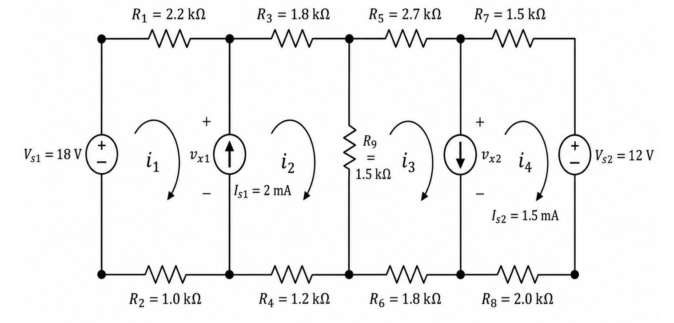
\includegraphics[width=0.70\columnwidth]{supermalla}
\caption{Circuito propuesto para análisis por supermallas}
\label{fig:supermalla}
\end{figure}

\subsection{Datos del circuito}

\begin{align*}
    R_1 &= 2.2k\Omega \\
    R_2 &= 1.0k\Omega \\
    R_3 &= 1.8k\Omega \\
    R_4 &= 1.2k\Omega \\
    R_5 &= 2.7k\Omega \\
    R_6 &= 1.8k\Omega \\
    R_7 &= 1.5k\Omega \\
    R_8 &= 2.0k\Omega \\
    R_9 &= 1.5k\Omega
\end{align*}

\begin{align*}
    V_{s1} &= 18V \\
    V_{s2} &= 12V
\end{align*}

\begin{align*}
    I_{s1} &= 2mA \\
    I_{s2} &= 1.5mA
\end{align*}

\subsection{Calculos Matematicos}

\subsubsection{Cálculos del Circuito}

\paragraph{Ecuaciones Principales}
\begin{align*}
    I_2 - I_1 &= 2\text{ mA} \quad &\text{Ec1} \\
    I_3 - I_4 &= 1.5\text{ mA} \quad &\text{Ec2}
\end{align*}

\paragraph{Supermalla 1 (Izquierda)}
\begin{align*}
    -18 + 2.2I_1 + 1I_1 + 1.8I_2 + 1.2I_2 + 1.5(I_2 - I_3) &= 0 \\
    3.2I_1 + 4.5I_2 - 1.5I_3 &= 18 \quad \text{Ec3}
\end{align*}

\paragraph{Supermalla 2 (Derecha)}
\begin{align*}
    1.5I_4 + 12 + 2I_4 + 1.8I_3 + 1.5(I_3 - I_2) + 2.7I_3 &= 0 \\
    3.5I_4 + 6I_3 - 1.5I_2 &= -12 \quad \text{Ec4}
\end{align*}

Sustituyendo las corrientes de las fuentes:
\begin{align*}
    I_2 &= 2 + I_1 \\
    I_4 &= I_3 - 1.5
\end{align*}

Reemplazando en las ecuaciones de las supermallas:
\begin{align*}
    3.2I_1 + 4.5(2 + I_1) - 1.5I_3 &= 18 \\
    3.5(I_3 - 1.5) + 6I_3 - 1.5(2 + I_1) &= -12 \\
    \\
    3.2I_1 + 9 + 4.5I_1 - 1.5I_3 &= 18 \\
    3.5I_3 - 5.25 + 6I_3 - 3 - 1.5I_1 &= -12 \\
    \\
    7.7I_1 - 1.5I_3 &= 18 - 9 \\
    9.5I_3 - 1.5I_1 &= -12 + 8.25
\end{align*}

\paragraph{Eliminación Multiplicando}
Sistema resultante:
\begin{align*}
    7.7I_1 - 1.5I_3 &= 9 \quad &\times (9.5) \\
    -1.5I_1 + 9.5I_3 &= -3.75 \quad &\times (1.5)
\end{align*}

Operando:
\begin{align*}
    73.15I_1 - 14.25I_3 &= 85.5 \\
    -2.25I_1 + 14.25I_3 &= -5.625 \\
    \hline
    70.9I_1 &= 79.875
\end{align*}

Despejando las corrientes:
\begin{align*}
    I_1 &= \frac{79.875}{70.9} \implies \mathbf{I_1 = 1.126\text{ mA}} \\
    \\
    I_2 &= 2 + 1.126 \implies \mathbf{I_2 = 3.126\text{ mA}} \\
    \\
    7.7(1.126) - 1.5I_3 &= 9 \\
    8.6702 - 9 &= 1.5I_3 \\
    \frac{-0.3298}{1.5} &= I_3 \implies \mathbf{I_3 = -0.219\text{ mA}} \\
    \\
    I_4 &= -0.219 - 1.5 \implies \mathbf{I_4 = -1.719\text{ mA}}
\end{align*}

\paragraph{Voltajes}
Cálculo de $V_{x1}$:
\begin{align*}
    -18 + 2.2I_1 + 1I_1 + V_{x1} &= 0 \\
    V_{x1} &= 18 - 3.2I_1 \\
    V_{x1} &= 18 - 3.2(1.126) \\
    V_{x1} &= 18 - 3.6032 \\
    \mathbf{V_{x1}} &\mathbf{= 14.3968\text{ V}}
\end{align*}

Cálculo de $V_{x2}$:
\begin{align*}
    12 + 1.5I_4 + 2I_4 - V_{x2} &= 0 \\
    V_{x2} &= 12 + 3.5I_4 \\
    V_{x2} &= 12 + 3.5(-1.719) \\
    V_{x2} &= 12 - 6.0165 \\
    \mathbf{V_{x2}} &\mathbf{= 5.9835\text{ V}}
\end{align*}

\subsection{Simulación}
El circuito fue simulado utilizando el software \textit{SimulIDE}, obteniendo resultados que se 
compararán con los cálculos teóricos realizados mediante el método de supermallas.

\begin{figure}[H]
\centering
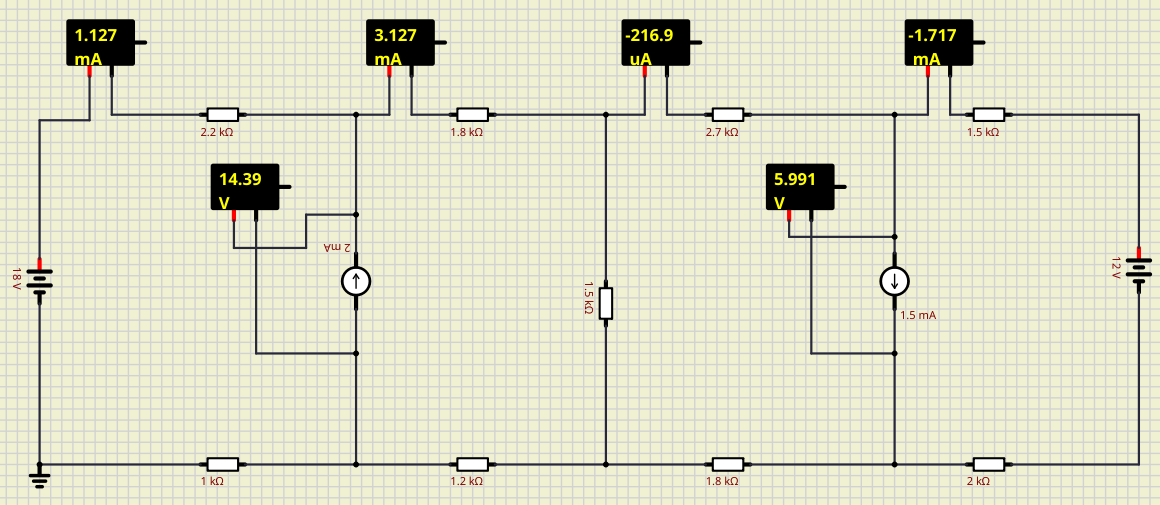
\includegraphics[width=0.70\columnwidth]{simulacion_supermalla.png}
\caption{Simulación del circuito mediante análisis por supermallas}
\end{figure}

\subsection{Tabla de resultados}

\begin{table}[h]
\centering
\caption{Comparación entre resultados teóricos y simulados (Ejercicio 1)}
\begin{tabular}{|c|c|c|c|c|}
\hline
\textbf{Variable} & \textbf{Teórico} & \textbf{Simulado} & \textbf{Error \%} & \textbf{Observación} \\
\hline
$I_1$ & $1.126 \text{ mA}$ & $1.127 \text{ mA}$ & $0.09\%$ & Correlación alta \\
\hline
$I_2$ & $3.126 \text{ mA}$ & $3.127 \text{ mA}$ & $0.03\%$ & Correlación alta \\
\hline
$I_3$ & $-0.219 \text{ mA}$ & $-0.2169 \text{ mA}$* & $0.96\%$ & Correlación alta \\
\hline
$I_4$ & $-1.719 \text{ mA}$ & $-1.717 \text{ mA}$ & $0.12\%$ & Correlación alta \\
\hline
$V_{x1}$ & $14.3968 \text{ V}$ & $14.39 \text{ V}$ & $0.05\%$ & Correlación alta \\
\hline
$V_{x2}$ & $5.9835 \text{ V}$ & $5.991 \text{ V}$ & $0.13\%$ & Correlación alta \\
\hline
\end{tabular}
\begin{flushleft}
\small *Valor convertido de $-216.9 \mu\text{A}$ obtenido en la simulación.
\end{flushleft}
\end{table}

\section{Ejercicio 2: Método de análisis nodal}

\subsection{Planteamiento}

Se analiza el circuito mostrado en la Fig.~\ref{fig:nodal} utilizando el método de análisis nodal 
para determinar los voltajes $V_a$, $V_b$ y $V_c$ respecto a tierra.

\begin{figure}[H]
\centering
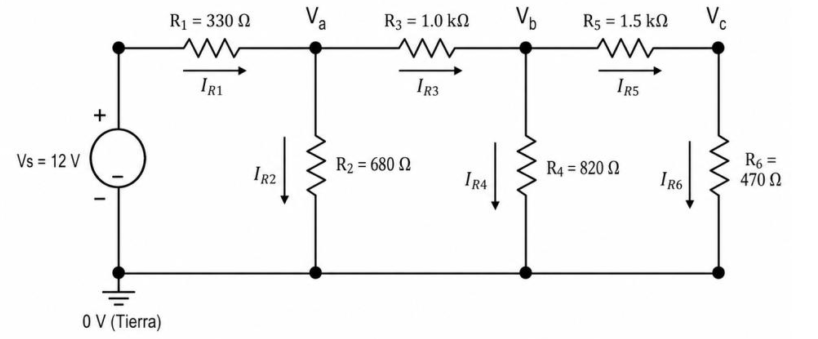
\includegraphics[width=0.70\columnwidth]{nodal}
\caption{Circuito propuesto para análisis nodal}
\label{fig:nodal}
\end{figure}

\subsection{Datos del circuito}

\begin{align*}
V_s &= 9V \\
R_1 &= 330\Omega \\
R_2 &= 680\Omega \\
R_3 &= 1k\Omega \\
R_4 &= 820\Omega \\
R_5 &= 1.5k\Omega \\
R_6 &= 470\Omega
\end{align*}

\subsection{Cálculos matemáticos}

Los nodos desconocidos son:

\begin{align*}
V_a,\;V_b,\;V_c
\end{align*}

\subsubsection{Ecuación nodal en $V_a$}

Aplicando Ley de Corrientes de Kirchhoff:

\begin{align*}
\frac{V_a-9}{330}+\frac{V_a}{680}+\frac{V_a-V_b}{1000}=0
\end{align*}

Multiplicando toda la ecuación por 2244000:

\begin{align*}
6800(V_a-9)+3300V_a+2244(V_a-V_b)=0
\end{align*}

Distribuyendo:

\begin{align*}
6800V_a-61200+3300V_a+2244V_a-2244V_b=0
\end{align*}

Agrupando términos semejantes:

\begin{align*}
12344V_a-2244V_b=61200
\end{align*}

\subsubsection{Ecuación nodal en $V_b$}

\begin{align*}
\frac{V_b-V_a}{1000}+\frac{V_b}{820}+\frac{V_b-V_c}{1500}=0
\end{align*}

Multiplicando toda la ecuación por 615000:

\begin{align*}
615(V_b-V_a)+750V_b+410(V_b-V_c)=0
\end{align*}

Distribuyendo:

\begin{align*}
615V_b-615V_a+750V_b+410V_b-410V_c=0
\end{align*}

Agrupando términos semejantes:

\begin{align*}
-615V_a+1775V_b-410V_c=0
\end{align*}

\subsubsection{Ecuación nodal en $V_c$}

\begin{align*}
\frac{V_c-V_b}{1500}+\frac{V_c}{470}=0
\end{align*}

Multiplicando toda la ecuación por 705000:

\begin{align*}
470(V_c-V_b)+1500V_c=0
\end{align*}

Distribuyendo:

\begin{align*}
470V_c-470V_b+1500V_c=0
\end{align*}

Agrupando términos semejantes:

\begin{align*}
-470V_b+1970V_c=0
\end{align*}

\subsubsection{Sistema de ecuaciones}

\begin{align*}
12344V_a-2244V_b&=61200 \\
-615V_a+1775V_b-410V_c&=0 \\
-470V_b+1970V_c&=0
\end{align*}

\subsubsection{Despeje de $V_c$}

De la tercera ecuación:

\begin{align*}
1970V_c&=470V_b
\end{align*}

\begin{align*}
V_c&=\frac{470V_b}{1970}
\end{align*}

\begin{align*}
V_c&=0.2386V_b
\end{align*}

\subsubsection{Sustitución en la segunda ecuación}

\begin{align*}
-615V_a+1775V_b-410(0.2386V_b)=0
\end{align*}

\begin{align*}
-615V_a+1775V_b-97.826V_b=0
\end{align*}

\begin{align*}
-615V_a+1677.174V_b=0
\end{align*}

Despejando $V_b$:

\begin{align*}
1677.174V_b&=615V_a
\end{align*}

\begin{align*}
V_b&=\frac{615V_a}{1677.174}
\end{align*}

\begin{align*}
V_b&=0.3667V_a
\end{align*}

\subsubsection{Sustitución en la primera ecuación}

\begin{align*}
12344V_a-2244(0.3667V_a)=61200
\end{align*}

\begin{align*}
12344V_a-822.8748V_a=61200
\end{align*}

\begin{align*}
11521.1252V_a=61200
\end{align*}

\begin{align*}
V_a=\frac{61200}{11521.1252}
\end{align*}

\begin{align*}
V_a=5.31V
\end{align*}

\subsubsection{Cálculo de $V_b$}

\begin{align*}
V_b=0.3667(5.31)
\end{align*}

\begin{align*}
V_b=1.95V
\end{align*}

\subsubsection{Cálculo de $V_c$}

\begin{align*}
V_c=0.2386(1.95)
\end{align*}

\begin{align*}
V_c=0.47V
\end{align*}

\subsubsection{Cálculo de corrientes}

\subsubsection{$I_{R1}$}

\begin{align*}
I_{R1}=\frac{9-5.31}{330}
\end{align*}

\begin{align*}
I_{R1}=0.01118A
\end{align*}

\begin{align*}
I_{R1}=11.18mA
\end{align*}

\subsubsection{$I_{R2}$}

\begin{align*}
I_{R2}=\frac{5.31}{680}
\end{align*}

\begin{align*}
I_{R2}=0.00781A
\end{align*}

\begin{align*}
I_{R2}=7.81mA
\end{align*}

\subsubsection{$I_{R3}$}

\begin{align*}
I_{R3}=\frac{5.31-1.95}{1000}
\end{align*}

\begin{align*}
I_{R3}=0.00336A
\end{align*}

\begin{align*}
I_{R3}=3.36mA
\end{align*}

\subsubsection{$I_{R4}$}

\begin{align*}
I_{R4}=\frac{1.95}{820}
\end{align*}

\begin{align*}
I_{R4}=0.00238A
\end{align*}

\begin{align*}
I_{R4}=2.38mA
\end{align*}

\subsubsection{$I_{R5}$}

\begin{align*}
I_{R5}=\frac{1.95-0.47}{1500}
\end{align*}

\begin{align*}
I_{R5}=0.00099A
\end{align*}

\begin{align*}
I_{R5}=0.99mA
\end{align*}

\subsubsection{$I_{R6}$}

\begin{align*}
I_{R6}=\frac{0.47}{470}
\end{align*}

\begin{align*}
I_{R6}=0.001A
\end{align*}

\begin{align*}
I_{R6}=1.00mA
\end{align*}

\subsubsection{Resultados finales}

Los voltajes nodales obtenidos fueron:

\begin{align*}
V_a &= 5.31V \\
V_b &= 1.95V \\
V_c &= 0.47V
\end{align*}

Las corrientes calculadas fueron:

\begin{align*}
I_{R1} &= 11.18mA \\
I_{R2} &= 7.81mA \\
I_{R3} &= 3.36mA \\
I_{R4} &= 2.38mA \\
I_{R5} &= 0.99mA \\
I_{R6} &= 1.00mA
\end{align*}

\subsection{Simulación}

El circuito fue simulado utilizando el software \textit{SimulIDE}, obteniendo resultados muy cercanos a los cálculos teóricos realizados mediante análisis nodal.

\begin{figure}[H]
\centering
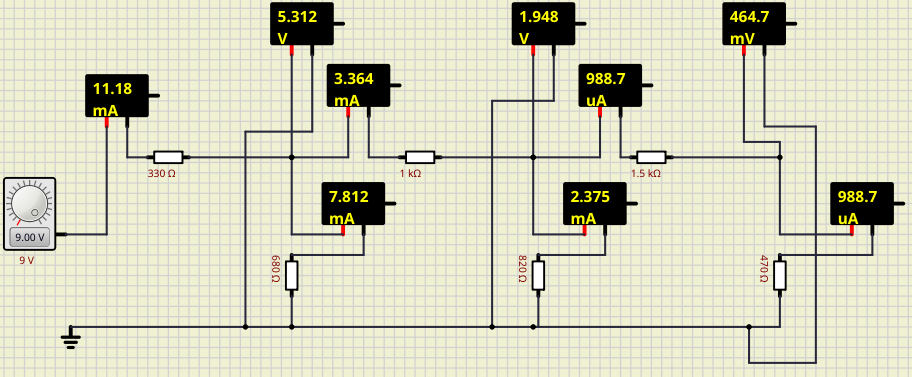
\includegraphics[width=0.70\columnwidth]{simulacion2.png}
\caption{Simulación del circuito mediante análisis nodal}
\end{figure}

\subsubsection{Resultados obtenidos en simulación}

\begin{align*}
V_a &= 5.312V \\
V_b &= 1.958V \\
V_c &= 0.4647V \\
I_{R1} &= 11.18mA \\
I_{R2} &= 7.812mA \\
I_{R3} &= 3.364mA \\
I_{R4} &= 2.375mA \\
I_{R5} &= 0.9887mA \\
I_{R6} &= 0.9887mA
\end{align*}

\subsection{Montaje físico}

Se realizó el montaje físico del circuito utilizando una protoboard, resistencias comerciales y una 
batería de $9V$ como fuente de alimentación.
%Suba la imagen del montaje del circuito por analisis nodal y le pone montaje nodal, THX
%\begin{figure}[H]
%\centering
%\includegraphics[width=0.48\columnwidth]{montaje_nodal}
%\caption{Montaje físico del circuito}
%\end{figure}

\subsection{Mediciones}

Las mediciones de voltaje y corriente se realizaron utilizando un multímetro digital.
%Suba las imágenes de las mediciones realizadas en el circuito y le pone mediciones nodal, THX
%\begin{figure}[H]
%\centering
%\includegraphics[width=0.32\columnwidth]{medicion}
%\caption{Mediciones realizadas en el circuito}
%\end{figure}

\subsubsection{Resultados medidos}

\begin{align*}
V_a &= 0V \\
V_b &= 0V \\
V_c &= 0V \\
I_{R1} &= 0mA \\
I_{R2} &= 0mA \\
I_{R3} &= 0mA \\
I_{R4} &= 0mA \\
I_{R5} &= 0mA \\
I_{R6} &= 0mA
\end{align*}

\subsection{Tabla de resultados}
Esta es la tabla de comparación entre los resultados teóricos, simulados y medidos, incluyendo los errores porcentuales entre cada método:
\begin{table}[h]
\centering
\caption{Comparación entre resultados teóricos, simulados y medidos}
\begin{tabular}{|c|c|c|c|c|c|}
\hline
\textbf{Variable} & \textbf{Teórico} & \textbf{Simulado} & \textbf{Medido} & \textbf{Error sim. \%} & \textbf{Error med. \%} \\
\hline
$V_a$ & $5.31V$ & $5.312V$ & & & \\
\hline
$V_b$ & $1.95V$ & $1.958V$ & & & \\
\hline
$V_c$ & $0.47V$ & $0.4647V$ & & & \\
\hline
$I_{R1}$ & $11.18mA$ & $11.18mA$ & & & \\
\hline
$I_{R2}$ & $7.81mA$ & $7.812mA$ & & & \\
\hline
$I_{R3}$ & $3.36mA$ & $3.364mA$ & & & \\
\hline
$I_{R4}$ & $2.38mA$ & $2.375mA$ & & & \\
\hline
$I_{R5}$ & $0.99mA$ & $0.9887mA$ & & & \\
\hline
$I_{R6}$ & $1.00mA$ & $0.9887mA$ & & & \\
\hline
\end{tabular}
\end{table}

\end{document}
